\documentclass{article}

\usepackage{neurips_2026}

\usepackage[utf8]{inputenc}
\usepackage[T1]{fontenc}
\usepackage{hyperref}
\usepackage{url}
\usepackage{booktabs}
\usepackage{amsfonts}
\usepackage{amsmath}
\usepackage{nicefrac}
\usepackage{microtype}
\usepackage{xcolor}
\usepackage{graphicx}
\usepackage{multirow}
\usepackage{subcaption}
\usepackage{tikz}
\usepackage{float}
\usetikzlibrary{positioning,arrows.meta,fit,calc,backgrounds,shapes.geometric,decorations.pathreplacing}

% Legacy macro (kept for backwards compatibility; new framing avoids a single named method).
\newcommand{\ours}{VoteAlign}
\newcommand{\todo}[1]{\textcolor{red}{[TODO: #1]}}
\newcommand{\placeholder}[1]{\textcolor{blue}{#1}}

\title{Pseudo-Gloss Conditioning and Denoiser Design for Diffusion-based Sign Language Production}

\author{%
  Anonymous Author(s)
}

\begin{document}

\maketitle

\begin{abstract}
Generating natural avatar motion from spoken-language text is a challenging multi-modal task that spans linguistic structure (gloss-level segmentation, sign-language word order) and high-dimensional motion synthesis.
We present a systematic study of two complementary design axes for diffusion-based sign language production (SLP):
\emph{(i)~conditioning input}---comparing sentence encoding, rule-based and LLM-drafted pseudo-glosses, token-level voting gates, cross-attention fusion, and SignBank phonological-attribute augmentation; and
\emph{(ii)~denoiser architecture}---we keep the MDM diffusion framework~\citep{tevet2023human} (cosine schedule, DDIM sampling, $\epsilon$-prediction) with sign-language-specific loss reweighting, and introduce two new variants of its transformer-encoder denoiser: a \emph{temporal-bias} variant (kin) that injects temporal locality through a learned pairwise frame bias on the relative time offset (shared across all layers and heads), and a \emph{multi-scale} variant (ms) that runs a coarse pooled stream in parallel with the fine-resolution stream to capture both short-range articulation and long-range phrase structure.
Across How2Sign (ASL) and PHOENIX-2014T (DGS), no single combination dominates universally:
kin with LLM-drafted gloss, token voting, and phonological attributes wins How2Sign (FID \textbf{1.94} / FID\textsubscript{AE} \textbf{1.19}, a $4.7\times$ FID\textsubscript{AE} reduction over the same denoiser without phonological attributes), while ms with token voting on ground-truth gloss wins PHOENIX-2014T (FID \textbf{21.81} / FID\textsubscript{AE} \textbf{6.28}).
We release all code, splits, evaluation pipelines, and trained checkpoints to support reproducible benchmarking in sign language production.
\end{abstract}

%=====================================================================
\section{Introduction}
\label{sec:intro}

Sign languages are full natural languages with their own grammar, syntax, and lexicon, distinct from their surrounding spoken languages~\citep{stokoe1960sign,sandler2006sign}.
Generating realistic avatar motion from spoken-language text---\emph{sign language production} (SLP)---is a step toward accessible communication technology, yet remains hampered by two coupled challenges.
First, sign languages convey meaning through the \emph{simultaneous} articulation of manual (handshape, location, movement) and non-manual (facial expression, body posture) channels~\citep{brentari1998prosodic}, demanding high-dimensional 3D motion representations.
Second, the mapping from spoken text to sign is not word-for-word: sign languages drop function words, employ different temporal ordering, and use spatial grammar that has no direct analog in spoken language~\citep{sandler2006sign}.

Diffusion-based approaches to SLP~\citep{hong2026phonologyguided} adapt the transformer-denoiser paradigm of MDM-style motion diffusion~\citep{tevet2023human} by conditioning on a sentence-level CLIP embedding, but this discards the discrete gloss-level structure that aligns with how signs are produced sequentially.
An alternative line of work is gloss-level conditioning~\citep{zheng2023sign2gpt,wong2025pgg}, which uses content words from the spoken sentence as a pseudo-gloss; existing methods extract these via either rule-based POS filtering~\citep{zheng2023sign2gpt} or LLM in-context learning~\citep{wong2025pgg}.
To date, no work has systematically studied how the choice of conditioning input interacts with the choice of denoiser architecture in the diffusion-based SLP setting, nor has the field consistently re-implemented and re-evaluated published baselines under a single controlled protocol.
Our motivating observation is that the two design choices---input and architecture---are not independent: a conditioning signal that helps one denoiser may hurt another, and a denoiser that wins on one dataset may lose on another.

We present such a study. We isolate two complementary design axes for diffusion-based SLP and study their interaction empirically:

\paragraph{Conditioning input.}
We compare six conditioning regimes under matched training and evaluation: (i)~sentence-only CLIP encoding; (ii)~rule-based pseudo-gloss; (iii)~LLM-drafted pseudo-gloss; (iv)~per-token voting gate that learns to weight or drop gloss tokens (\emph{VoteOnly}); (v)~per-frame cross-attention fusion of motion to gloss tokens (\emph{VoteAlign}); and (vi)~SignBank phonological-attribute augmentation that fuses handshape, location, movement, orientation, contact, and repetition tokens with each gloss embedding.

\paragraph{Denoiser architecture.}
We keep the MDM diffusion framework~\citep{tevet2023human} as our base, adapted to sign language with upper-body joints, joint-region weighted reconstruction loss, and CFG with $\epsilon$-prediction.
We then introduce two new variants of its transformer-encoder denoiser: a \emph{temporal-bias variant} (kin) that adds a learned pairwise frame bias on the relative time offset (shared across all layers and heads) to encode temporal locality, and a \emph{multi-scale variant} (ms) that runs a fine-resolution stream and a coarse pooled stream in parallel to capture both short-range articulation and long-range phrase structure.

We evaluate on How2Sign (American Sign Language, English) and PHOENIX-2014T (German Sign Language, German), under a unified self-contained protocol detailed in Section~\ref{sec:experiments}.
Our contributions are:
\begin{itemize}
    \item \textbf{Two new denoiser variants for SLP.} \emph{kin} adds a learnable relative-time bias to the pre-softmax attention logits (shared across all layers and heads), encoding a soft temporal-locality prior over frames; \emph{ms} runs a fine-resolution stream in parallel with a $2{\times}$ pooled coarse stream and sums their outputs, capturing short-range articulation and long-range phrase structure within the same parameter budget as the MDM baseline.
    \item \textbf{Two new gloss-conditioning modules and a phonological augmentation that composes with both.} \emph{VoteOnly} attaches a per-token learnable sigmoid keep/drop gate to LLM-drafted pseudo-glosses, refining the draft end-to-end through the diffusion loss without gloss-level supervision; \emph{VoteAlign} replaces the gate with cross-attention from motion frames to gloss tokens, producing per-frame conditioning that jointly performs token selection and temporal alignment without an explicit gate. A SignBank phonological-attribute augmentation fuses six handshape/location/movement attributes per gloss token and is composable with CFG, VoteOnly, and VoteAlign without changing their downstream interface.
    \item \textbf{Empirical insight: optimal combination is dataset-dependent.} Under our unified protocol, \textbf{kin $\cdot$ VoteOnly with LLM-drafted gloss and phonological attributes wins How2Sign} (FID \textbf{1.94} / FID\textsubscript{AE} \textbf{1.19}); \textbf{ms $\cdot$ VoteOnly with ground-truth gloss wins PHOENIX-2014T} (FID \textbf{21.81} / FID\textsubscript{AE} \textbf{6.28}). Across both datasets, token-level voting consistently outperforms the more complex cross-attention fusion, and phonological augmentation delivers a $4.7{\times}$ FID\textsubscript{AE} reduction on the kin denoiser specifically.
\end{itemize}

%=====================================================================
\section{Related Work}
\label{sec:related}

\paragraph{Sign language production.}
Sign language production (SLP) generates sign motion from text or gloss input.
Early methods use lookup-and-concatenate approaches~\citep{mcdonald2016automated} or statistical parametric synthesis~\citep{cox2002tessa}.
Progressive Transformers~\citep{saunders2020progressive,saunders2021continuous} autoregressively generate skeleton sequences conditioned on gloss input.
More recently, diffusion-based methods have shown promise: \citet{hong2026phonologyguided} establish a strong diffusion baseline using SMPL-X representation and systematically study phonological attribute conditioning, finding that input representation format significantly affects text-encoder-based conditioning.
SignDiff~\citep{fang2023signdiff} applies diffusion to sign pose generation.
T2S-GPT~\citep{xie2024t2sgpt} uses VQ-VAE with autoregressive generation.
However, these methods either condition on gold-standard glosses (unavailable at inference for novel sentences) or on full sentences (losing gloss-level structure).
Our work bridges this gap by learning to extract and align pseudo-glosses in an end-to-end framework.

\paragraph{Pseudo-gloss extraction for sign language.}
Extracting gloss-like representations from spoken-language text has been explored primarily for sign language \emph{translation} (video to text), not generation.
Sign2GPT~\citep{zheng2023sign2gpt} uses spaCy POS filtering to keep content words as pseudo-glosses, but retains spoken-language word order without reordering.
PGG-SLT~\citep{wong2025pgg} uses an LLM with in-context learning to draft pseudo-glosses, then trains a video frame-level classifier to reorder the draft into sign-language temporal order via a greedy algorithm.
Select and Reorder~\citep{walsh2024select} decouples text-to-gloss into selection and reordering stages with non-autoregressive decoding, but only targets text-to-gloss without downstream motion generation.
Our approach differs in three key ways: (1)~we target the generation direction (text to motion), (2)~we use motion features rather than video features, and (3)~we replace explicit reordering with implicit cross-attention alignment, enabling end-to-end training through the generation objective.

\paragraph{Diffusion models for human motion.}
MDM~\citep{tevet2023human} introduces a transformer-based diffusion model for text-conditioned human motion generation.
MLD~\citep{chen2023mld} operates in a latent space for efficiency.
MotionDiffuse~\citep{zhang2022motiondiffuse} enables fine-grained text-motion control.
These methods typically use a single sentence embedding as condition, prepended as a token to the denoising transformer.
Our work extends this paradigm by introducing per-frame cross-attention conditioning from gloss tokens, enabling temporally-varying control that is particularly important for sign language where different glosses correspond to different temporal segments.

\paragraph{Cross-attention for temporal alignment.}
Cross-attention as a mechanism for learning alignment between sequences is well-established in machine translation~\citep{vaswani2017attention,bahdanau2015neural}, where it naturally handles word-order differences between languages.
In motion generation, Make-An-Animation~\citep{azadi2024make} and TEMOS~\citep{petrovich2022temos} use cross-attention for text-motion alignment, but at the sentence level.
We apply cross-attention specifically for \emph{gloss-level} temporal alignment in sign language, where the ordering difference between spoken and signed forms is linguistically motivated and systematic.


%=====================================================================
\section{Method}
\label{sec:method}

% ===================== ARCHITECTURE FIGURE =====================
% Common tikz styles (reused across both subfigures)
\tikzset{
    >=Stealth,
    archstyles/.style={
        node distance=0.4cm and 0.6cm,
    },
    frozen/.style={draw, thick, rounded corners=3pt, minimum height=0.65cm,
                   align=center, font=\scriptsize, fill=gray!22, dashed,
                   minimum width=2.6cm},
    sentmod/.style={draw, thick, rounded corners=3pt, minimum height=0.65cm,
                    align=center, font=\scriptsize, fill=cyan!28,
                    minimum width=2.6cm},
    glossmod/.style={draw, thick, rounded corners=3pt, minimum height=0.65cm,
                     align=center, font=\scriptsize, fill=blue!22,
                     minimum width=2.6cm},
    phonomod/.style={draw, thick, rounded corners=3pt, minimum height=0.65cm,
                     align=center, font=\scriptsize, fill=violet!28,
                     minimum width=2.6cm},
    condblock/.style={draw, very thick, rounded corners=4pt, minimum height=0.95cm,
                      align=center, font=\small, fill=yellow!18,
                      minimum width=2.7cm},
    fusionmod/.style={draw, thick, rounded corners=3pt, minimum height=0.85cm,
                      align=center, font=\footnotesize, fill=orange!22,
                      minimum width=4.8cm},
    denoisermod/.style={draw, thick, rounded corners=3pt, minimum height=0.8cm,
                        align=center, font=\footnotesize, fill=green!22,
                        minimum width=4.8cm},
    projmod/.style={draw, thick, rounded corners=3pt, minimum height=0.65cm,
                    align=center, font=\scriptsize, fill=purple!18,
                    minimum width=2.6cm},
    data/.style={font=\footnotesize, align=center},
    tensor/.style={draw, rounded corners=2pt, fill=white, font=\scriptsize,
                   align=center, minimum height=0.5cm, inner sep=2.5pt,
                   minimum width=2.0cm},
    condout/.style={draw, rounded corners=2pt, font=\footnotesize, align=center,
                    minimum height=0.55cm, inner sep=3pt, minimum width=1.6cm},
    arrow/.style={->, thick, >=Stealth},
    optarrow/.style={->, thick, >=Stealth, dashed, gray!75},
    plugbox/.style={draw, thick, densely dashed, rounded corners=8pt,
                    fill=yellow!7, inner sep=8pt, line width=0.7pt},
}

\begin{figure}[t]
\centering

% ===================================================================
% PANEL (a) MAIN PIPELINE
% ===================================================================
\begin{subfigure}[t]{0.42\textwidth}
\centering
\resizebox{\textwidth}{!}{%
\begin{tikzpicture}[archstyles]

% Top: noisy motion input
\node[data] (motin) at (0, 0) {Noisy motion $\mathbf{x}_t$,\; timestep $t$};

% ---- Diffusion core (middle) ----
\node[fusionmod, below=0.5cm of motin, minimum width=3.8cm] (xattn)
    {\textbf{Cross-Attention Fusion}};
\draw[arrow] (motin) -- node[right, font=\scriptsize, xshift=1pt] {Q} (xattn);

% Conditioning enters from the right (output of panel (b))
\node[data, anchor=west, font=\footnotesize, align=left]
    (cext) at ([xshift=0.55cm]xattn.east)
    {$\mathbf{c}$\\[-2pt]{\scriptsize from (b)}};
\draw[arrow] (cext.west) -- node[above, font=\scriptsize] {K/V} (xattn.east);

% Per-frame features
\node[tensor, below=0.3cm of xattn, minimum width=3.5cm] (ff)
    {Per-frame features $\mathbf{f}_1,\ldots,\mathbf{f}_T$};
\draw[arrow] (xattn) -- (ff);

% Denoiser (one of MDM / kin / ms — see Section~\ref{sec:backbones})
\node[denoisermod, below=0.3cm of ff, minimum width=3.8cm] (denoiser)
    {\textbf{Denoiser}};
\draw[arrow] (ff) -- (denoiser);

% Output at the bottom
\node[condout, below=0.3cm of denoiser, fill=green!10, minimum width=3.2cm] (eps)
    {Predicted noise $\hat{\boldsymbol{\epsilon}}$};
\draw[arrow] (denoiser) -- (eps);

\end{tikzpicture}
}%
\caption{\textbf{Main pipeline.} $\mathbf{x}_t$ queries cross-attention; condition tokens $\mathbf{c}$ from panel~(b) supply the keys/values. Motion projection and timestep embedding are omitted.}
\label{fig:arch_main}
\end{subfigure}%
\hfill
% ===================================================================
% PANEL (b) CONDITIONING DETAIL
% ===================================================================
\begin{subfigure}[t]{0.56\textwidth}
\centering
\resizebox{\textwidth}{!}{%
\begin{tikzpicture}[archstyles]

\def\Xs{-3.1}
\def\Xg{0}
\def\Xp{3.1}

% Top input
\node[data] (sin_d) at (\Xg, 0) {Spoken-language sentence $s$};

% Gloss branch (middle)
\node[frozen, below=0.5cm of sin_d] (llm_d) {Frozen LLM\\{\scriptsize(Qwen2.5-32B)}};
\draw[arrow] (sin_d) -- (llm_d);

\node[tensor, below=of llm_d, minimum width=2.6cm] (gtok_d)
    {$g_1, g_2, \ldots, g_K$};
\draw[arrow] (llm_d) -- (gtok_d);

\node[frozen, below=of gtok_d] (clip_g_d) {Frozen text encoder\\{\scriptsize(per-word)}};
\draw[arrow] (gtok_d) -- (clip_g_d);

\node[condout, below=of clip_g_d, fill=blue!14] (cgloss_d)
    {$\mathbf{c}^{\mathrm{gloss}}_{1..K}$};
\draw[arrow] (clip_g_d) -- (cgloss_d);

% Sentence branch (left)
\node[frozen] (clip_s_d) at ($(llm_d) + (\Xs, 0)$) {Frozen text encoder\\{\scriptsize(whole sentence, shared)}};
\draw[arrow] (sin_d.south) -- ++(0,-0.15) -| (clip_s_d.north);

\node[tensor] (efeat_d) at ($(gtok_d) + (\Xs, 0)$)
    {$\mathbf{e}^{s}_{1}, \ldots, \mathbf{e}^{s}_{L}$};
\draw[arrow] (clip_s_d) -- (efeat_d);

\node[sentmod] (sentenc_d) at ($(clip_g_d) + (\Xs, 0)$) {\textbf{MLP}};
\draw[arrow] (efeat_d) -- (sentenc_d);

\node[condout, fill=cyan!18] (csent_d) at ($(cgloss_d) + (\Xs, 0)$)
    {$\mathbf{c}^{\mathrm{sent}}$};
\draw[arrow] (sentenc_d) -- (csent_d);

% Phono branch (right, from gtok_d): per-gloss attribute lookup [How2Sign-only, dashed frame]
\node[frozen] (lex_d) at ($(gtok_d) + (\Xp, 0)$)
    {ASL-SignBank Lookup\\{\scriptsize Hand / Loc / Mvmt attrs}};
\draw[arrow] (gtok_d.east) -- (lex_d.west);

\node[frozen] (phonoenc_d) at ($(clip_g_d) + (\Xp, 0)$)
    {Frozen text encoder\\{\scriptsize(per-attribute)}};
\draw[arrow] (lex_d) -- (phonoenc_d);

\node[condout, fill=violet!18] (cphono_d) at ($(cgloss_d) + (\Xp, 0)$)
    {$\mathbf{c}^{\mathrm{phono}}_{1..K}$};
\draw[arrow] (phonoenc_d) -- (cphono_d);

% Dashed frame around phono branch (How2Sign-only)
\begin{scope}[on background layer]
    \node[draw, dashed, thick, rounded corners=4pt, inner sep=5pt,
          fit=(lex_d)(phonoenc_d)(cphono_d)] (phonobox_d) {};
\end{scope}
\node[font=\scriptsize\itshape, anchor=south, yshift=1pt]
    at (phonobox_d.north) {How2Sign only};

% Condition tokens output: widened to span all three column outputs.
\node[condout, fill=yellow!28, minimum width=10.5cm, minimum height=0.7cm, font=\small]
    at ($(cgloss_d.south) + (0,-0.75)$) (cfinal_d)
    {Condition tokens $\mathbf{c} \in \bigl\{\,\mathbf{c}^{\mathrm{sent}},\; \mathbf{c}^{\mathrm{gloss}}_{1..K},\; \mathbf{c}^{\mathrm{phono}}_{1..K}\,\bigr\}$};
\draw[arrow] (csent_d.south)  -- (csent_d.south  |- cfinal_d.north);
\draw[arrow] (cgloss_d.south) -- (cgloss_d.south |- cfinal_d.north);
\draw[arrow] (cphono_d.south) -- (cphono_d.south |- cfinal_d.north);

% Pluggable conditioning box
\begin{scope}[on background layer]
    \node[plugbox, fit=(sin_d)(clip_s_d)(llm_d)(lex_d)(csent_d)(cgloss_d)(cphono_d)(cfinal_d)(phonobox_d)] (plugbox_d) {};
\end{scope}

\end{tikzpicture}
}%
\caption{\textbf{Pluggable Conditioning.} Three parallel branches produce three candidate condition-token sources; exactly one is enabled per experiment and fed to the cross-attention fusion in~(a) as keys/values. Phono branch (dashed) is How2Sign only.}
\label{fig:arch_detail}
\end{subfigure}

\caption{\textbf{Overall architecture (dataset-agnostic structure).}
(a)~Compact main pipeline: $\mathbf{x}_t$ is fed as queries to a \textcolor{orange!80!black}{cross-attention fusion} module with $\mathbf{c}$ as keys/values, followed by a \textcolor{green!50!black}{denoiser} (one of MDM / kin / ms; Section~\ref{sec:backbones}) predicting $\hat{\boldsymbol{\epsilon}}$. Motion is SMPL-X axis-angle for How2Sign ($D{=}159$) and 2D upper-body MediaPipe joints for PHOENIX-2014T ($D{=}201$); the rest of the pipeline is identical.
(b)~Three parallel branches define three candidate condition-token sources, exactly one of which is enabled per experiment. \textit{Sentence:} frozen text encoder + trainable MLP. \textit{Gloss:} frozen LLM drafts pseudo-glosses, embedded per-word by a shared frozen text encoder; the resulting per-word embeddings $\mathbf{c}^{\mathrm{gloss}}_{1..K}$ are passed downstream to the conditioning module of choice (CFG / VoteOnly / VoteAlign in Section~\ref{sec:voting}--\ref{sec:fusion}), where the trainable transformer encoder + voting/fusion produces the final condition. \textit{Phonological (dashed frame, How2Sign only):} each gloss is queried in ASL-SignBank for its handshape/location/movement attributes; the resulting attribute words are embedded by the same frozen text encoder used in the gloss branch, producing $\mathbf{c}^{\mathrm{phono}}_{1..K}$. \textbf{This branch exists only for How2Sign}; PHOENIX-2014T has no analogous DGS phonological lexicon, so the phonology branch is omitted entirely on Phoenix and its conditioning set reduces to $\{\mathbf{c}^{\mathrm{sent}},\; \mathbf{c}^{\mathrm{gloss}}_{1..K}\}$. (How $\mathbf{c}^{\mathrm{phono}}_{1..K}$ is combined with the gloss tokens is described in Section~\ref{sec:phonology}; the figure deliberately shows the three branches as parallel sources rather than committing to a particular fusion.)
The frozen text encoder is CLIP-ViT-B/32 for How2Sign (English) and XLM-RoBERTa-base~\citep{conneau2020xlmr} for PHOENIX-2014T (German; we shorthand it ``mclip'' for the multilingual conditioning role, but it is not a multilingual CLIP variant). For PHOENIX-2014T an additional \emph{gt} input variant feeds the dataset-provided gold-standard gloss directly through the gloss branch (without the LLM/rule extractor).}
\label{fig:architecture}
\end{figure}

\subsection{Overview}
\label{sec:overview}

Given a spoken-language sentence $s$, our goal is to generate a 3D sign-language motion sequence $\mathbf{x} = (\mathbf{x}_1, \ldots, \mathbf{x}_T) \in \mathbb{R}^{T \times D}$ via a conditional diffusion model. We organize our study along two design axes that can be combined freely:

\textbf{(I) Conditioning input}---how the input sentence $s$ is converted into a conditioning signal for the denoiser. We compare six options: sentence-level CLIP encoding, rule-based pseudo-gloss extraction, LLM-drafted pseudo-gloss (Section~\ref{sec:draft}), a learnable per-token voting gate (\emph{VoteOnly}, Section~\ref{sec:voting}), per-frame cross-attention fusion of motion to gloss tokens (\emph{VoteAlign}, Section~\ref{sec:fusion}), and SignBank phonological-attribute augmentation (Section~\ref{sec:phonology}).

\textbf{(II) Denoiser architecture}---the transformer-encoder core of the diffusion denoiser. We keep the MDM diffusion framework~\citep{tevet2023human} as our base, adapted for sign language, and introduce two new variants of its transformer-encoder denoiser: a \emph{temporal-bias} variant (\textbf{kin}) that injects a learned temporal-locality prior, and a \emph{multi-scale} variant (\textbf{ms}) that captures both short-range articulation and long-range phrase structure (Section~\ref{sec:backbones}).

Figure~\ref{fig:architecture} shows the overall pipeline. The conditioning module on the right (panel b) and the denoiser core on the left (panel a) are independently swappable: any conditioning option can be paired with any denoiser variant.

\subsection{Diffusion framework and denoiser variants}
\label{sec:backbones}

\paragraph{MDM-based diffusion framework.}
We adopt an MDM-style~\citep{tevet2023human} diffusion model in motion space. The framework uses a cosine noise schedule with $\mathcal{T}=1000$ training steps, $\epsilon$-prediction, DDIM sampling~\citep{song2021denoising} with $50$ inference steps, and classifier-free guidance (CFG)~\citep{ho2022classifier} with unconditional probability $p_{\text{uncond}}=0.1$ at training and guidance scale $w=3.0$ at inference. Motion is represented in SMPL-X axis-angle for How2Sign (53 upper-body joints, $D=159$) and as 2D upper-body MediaPipe joints for PHOENIX-2014T ($D=201$). The denoiser is trained with a joint-region weighted MSE loss:
\begin{equation}
    \mathcal{L} = \sum_{j \in \mathcal{J}} \lambda_j \cdot \text{MSE}_\text{masked}(\hat{\epsilon}_j, \epsilon_j),
\end{equation}
where $\mathcal{J}$ indexes joint groups (torso, arms, hands, jaw) with $\lambda_\text{torso}=0.5$, $\lambda_\text{arms}=\lambda_\text{lhand}=\lambda_\text{rhand}=5.0$, $\lambda_\text{jaw}=0.1$, and root / lower-body weights set to zero (we focus on upper-body signing). Masking accounts for variable-length sequences. CFG is applied at inference as
\begin{equation}
    \hat{\epsilon} = \epsilon_{\text{uncond}} + w \cdot (\epsilon_{\text{cond}} - \epsilon_{\text{uncond}}).
\end{equation}
All three denoiser variants below share these framework settings; they differ only in the transformer-encoder core (Figure~\ref{fig:denoisers}).

% ===================== FIGURE: 3 DENOISER VARIANTS =====================
\begin{figure}[t]
\centering
\tikzset{
    den_styles/.style={
        node distance=0.35cm,
        every node/.style={font=\footnotesize, align=center},
    },
    den_block/.style={draw, rounded corners=2pt, minimum width=2.6cm,
                      minimum height=0.55cm, fill=green!12},
    den_block_kin/.style={draw, rounded corners=2pt, minimum width=2.9cm,
                          minimum height=0.85cm, fill=blue!14, align=center},
    den_block_ms/.style={draw, rounded corners=2pt, minimum width=1.8cm,
                         minimum height=0.95cm, align=center},
    den_io/.style={draw, rounded corners=2pt, minimum width=2.6cm,
                   minimum height=0.5cm, font=\footnotesize},
    den_arrow/.style={->, thick, >=Stealth},
}

% Panel (a) MDM
\begin{subfigure}[t]{0.31\textwidth}
\centering
\begin{tikzpicture}[den_styles]
  \node[den_io] (in) {Motion features $\mathbf{x}$};
  \node[den_block, below=of in] (sa) {Self-Attention};
  \node[den_block, below=of sa] (ffn) {Feed-Forward};
  \node[font=\scriptsize, below=0.4cm of ffn] (rep) {$\times\, N{=}4$};
  \node[den_io, below=0.4cm of rep] (out) {Output $\mathbf{h}$};
  \draw[den_arrow] (in) -- (sa);
  \draw[den_arrow] (sa) -- (ffn);
  \draw[den_arrow] (ffn) -- (rep);
  \draw[den_arrow] (rep) -- (out);
\end{tikzpicture}
\caption{\textbf{MDM} (baseline).}
\label{fig:den_mdm}
\end{subfigure}%
\hfill
% Panel (b) kin
\begin{subfigure}[t]{0.31\textwidth}
\centering
\begin{tikzpicture}[den_styles]
  \node[den_io] (in) {Motion features $\mathbf{x}$};
  \node[den_block_kin, below=of in] (sa) {Self-Attention\\[-2pt]\scriptsize{$+\,b_{i-j}$ (rel-time bias)}};
  \node[den_block, below=of sa] (ffn) {Feed-Forward};
  \node[font=\scriptsize, below=0.4cm of ffn] (rep) {$\times\, N{=}4$};
  \node[den_io, below=0.4cm of rep] (out) {Output $\mathbf{h}$};
  \draw[den_arrow] (in) -- (sa);
  \draw[den_arrow] (sa) -- (ffn);
  \draw[den_arrow] (ffn) -- (rep);
  \draw[den_arrow] (rep) -- (out);
\end{tikzpicture}
\caption{\textbf{kin}: + relative-time bias.}
\label{fig:den_kin}
\end{subfigure}%
\hfill
% Panel (c) ms
\begin{subfigure}[t]{0.31\textwidth}
\centering
\begin{tikzpicture}[den_styles]
  \node[den_io] (in) {Motion features $\mathbf{x}$};
  \node[den_block_ms, fill=green!12, below=0.55cm of in, xshift=-1.05cm] (fine)
       {Fine TF\\\scriptsize $T$, $N/2{=}2$};
  \node[den_block_ms, fill=orange!22, below=0.55cm of in, xshift=1.05cm] (coarse)
       {Pool$2{\times}$\\Coarse TF\\Up$2{\times}$\\\scriptsize $T/2$, $N/2{=}2$};
  \node[circle, draw, fill=yellow!30, minimum size=0.5cm,
        below=0.4cm of in, yshift=-1.55cm] (sum) {$+$};
  \node[den_io, below=0.4cm of sum] (out) {LayerNorm $\to$ $\mathbf{h}$};
  \draw[den_arrow] (in.south) -- ++(0,-0.1) -| (fine.north);
  \draw[den_arrow] (in.south) -- ++(0,-0.1) -| (coarse.north);
  \draw[den_arrow] (fine.south) |- (sum.west);
  \draw[den_arrow] (coarse.south) |- (sum.east);
  \draw[den_arrow] (sum) -- (out);
\end{tikzpicture}
\caption{\textbf{ms}: fine + coarse streams.}
\label{fig:den_ms}
\end{subfigure}

\caption{\textbf{Three denoiser variants.} (a)~Vanilla MDM transformer-encoder denoiser ($N{=}4$ pre-norm encoder layers, $h{=}8$, $d_{\text{model}}{=}512$). (b)~\emph{kin} adds a learnable bias $b_{i-j}$ on relative time offset to the pre-softmax attention logits, shared across all layers and heads. (c)~\emph{ms} runs a fine-resolution stream and a $2{\times}$-pooled coarse stream in parallel ($N/2{=}2$ layers each, summed before LayerNorm). All three share input/output projections, layer count, hidden dim, and feed-forward width; only the transformer-encoder block differs.}
\label{fig:denoisers}
\end{figure}

\paragraph{Standard transformer denoiser (MDM).}
The default denoiser is a stack of $N{=}4$ pre-norm transformer encoder layers with $h{=}8$ heads, model dimension $d_{\text{model}}{=}512$, and feed-forward expansion $4\times$, identical to MDM~\citep{tevet2023human} modulo our sign-language-specific input dimension. Self-attention is unrestricted across frames; positional encoding is sinusoidal. We refer to this configuration as \textbf{MDM} in tables (consistent with the codebase \texttt{model\_arch=mdm} flag) and use it as the architectural baseline to which we compare kin and ms.

\paragraph{Temporal-bias variant (kin).}
The kin variant augments each layer's self-attention with a learnable pairwise frame bias $b_{ij}$ added to the pre-softmax attention logits, where $b_{ij}$ is a function of the relative time offset $i{-}j$ learned globally and shared across all layers and attention heads:
\begin{equation}
    \text{Attn}(Q,K,V)_{ij} = \text{softmax}_j\!\left(\frac{Q_i K_j^\top}{\sqrt{d_{\text{model}}}} + b_{ij}\right) V.
\end{equation}
Initializing $b_{ij}{=}0$ recovers MDM's vanilla attention; the bias is free to learn during training. The kin variant encodes a soft \emph{temporal locality} prior matched to sign-language articulation, where adjacent frames are more correlated than distant ones. The number of layers, heads, and feed-forward dimension match the MDM denoiser, so kin and MDM have nearly identical parameter counts.

\paragraph{Multi-scale variant (ms).}
The ms variant runs two parallel transformer streams over the noisy motion features: a \emph{fine} stream at full temporal resolution $T$, and a \emph{coarse} stream operating on the output of $2{\times}$ average-pooling along the time axis (length $T/2$). Each stream uses $N/2{=}2$ pre-norm transformer encoder layers (so the total parameter budget matches MDM's $4$-layer single stream). The coarse stream's outputs are nearest-neighbour upsampled back to length $T$ and summed with the fine stream's outputs, followed by a final layer norm:
\begin{equation}
    \mathbf{h} = \text{LayerNorm}\!\left(\text{TF}_{\text{fine}}(\mathbf{x}) + \text{Up}_{2\times}\!\left(\text{TF}_{\text{coarse}}(\text{Pool}_{2\times}(\mathbf{x}))\right)\right).
\end{equation}
The two scales correspond to two timescales relevant for sign language: short-range articulation within a single sign (handshape transition, contact event) and longer-range phrase-level structure (sign-to-sign timing, pause placement). The ms variant adds no additional parameters beyond redistributing the layer budget across the two streams.

\subsection{Pseudo-gloss draft via LLM}
\label{sec:draft}

A key challenge is converting spoken-language sentences into sign-appropriate conditioning tokens.
Rule-based extraction---POS filtering followed by lemmatization~\citep{zheng2023sign2gpt}---operates word-by-word: it keeps tokens whose POS tag is in a predefined content-word set (nouns, verbs, adjectives, adverbs) and lemmatizes the survivors.
While simple, this approach has two systematic failure modes.
First, it cannot reason about \emph{multi-word structures}: in ``We're going to be learning how to play Portal,'' the auxiliary chain ``are going to be'' should be dropped as a unit, but a POS tagger labels ``going'' as a verb and ``learning'' as a gerund, causing the rule-based method to retain both.
Second, it lacks \emph{contextual judgment}: structural ``how'' (``learn \emph{how to} play'' $\to$ drop) and interrogative ``how'' (``\emph{How} do we move?'' $\to$ keep) share the same POS tag but serve different functions.

We address these limitations with a frozen open-source LLM (Qwen2.5-32B-Instruct) prompted via few-shot in-context learning.
Following PGG-SLT~\citep{wong2025pgg}, we provide 31 hand-curated sentence--gloss pairs as demonstrations.
The prompt instructs the LLM to follow a three-step procedure:

\begin{enumerate}
    \item \textbf{Phrase-level chunking.} Identify multi-word structures \emph{before} analyzing individual words---auxiliary chains (``is going to,'' ``has been doing''), phrasal verbs (``break down,'' ``set up''), light verb constructions (``make sure'' $\to$ ``sure,'' ``take a look'' $\to$ ``look''), and discourse frames (``let me,'' ``you know'').
    This step prevents the ``going'' error described above.
    \item \textbf{Core meaning filtering.} Keep content words, pronouns, negations, WH-words, numbers, meaningful modals, and spatial/directional words; drop articles, copulas, auxiliaries, conjunctions, structural prepositions, degree modifiers (``very,'' ``really''), and discourse fillers.
    \item \textbf{Citation form restoration.} Lemmatize each retained word to its base form (``gives'' $\to$ ``give,'' ``children'' $\to$ ``child''), with an explicit guard against producing non-word fragments.
\end{enumerate}

Table~\ref{tab:gloss_examples} shows concrete examples comparing the two extraction methods.
The LLM correctly collapses auxiliary chains (row~1), drops structural ``how'' while retaining interrogative ``how'' (rows~1 vs.\ 2), and removes degree modifiers that ASL expresses through sign intensity rather than separate signs (row~3).
The full prompt and example list are provided in Appendix~\ref{app:llm_prompt}.

\begin{table}[h]
  \caption{\textbf{Rule-based vs.\ LLM-drafted pseudo-gloss extraction.} Errors in the rule-based output are \underline{underlined}.}
  \label{tab:gloss_examples}
  \centering
  \small
  \begin{tabular}{p{5.8cm}p{3.8cm}p{3.8cm}}
    \toprule
    \textbf{English sentence} & \textbf{Rule-based} & \textbf{LLM draft} \\
    \midrule
    Today we're going to be learning how to play Portal, a game by Valve Software.
      & today we \underline{go} \underline{learn} \underline{how} play portal game valve software
      & today we learn play portal game valve software \\[4pt]
    How do we move around in belly dance?
      & \underline{move} \underline{around} belly dance
      & how we move around belly dance \\[4pt]
    You will really start feeling the burn.
      & you \underline{really} start feel burn
      & you start feel burn \\
    \bottomrule
  \end{tabular}
\end{table}

All draft glosses are pre-computed offline and cached; the LLM incurs no cost during training or inference.

% ===================== COMPARISON FIGURE: VoteOnly vs VoteAlign =====================
\begin{figure}[t]
\centering
\begin{subfigure}[t]{0.48\textwidth}
\centering
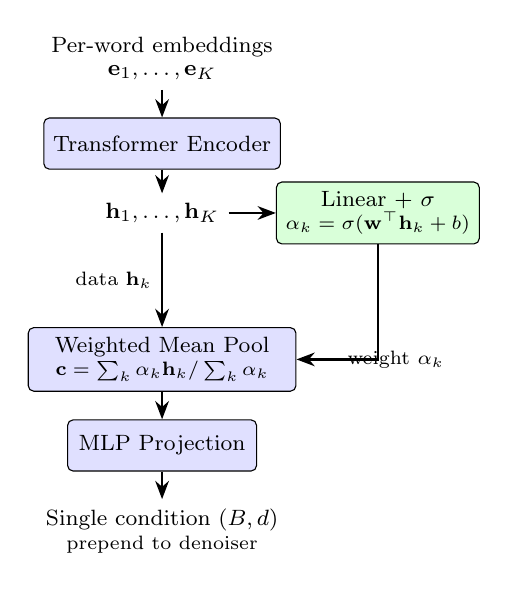
\begin{tikzpicture}[
    >=Stealth,
    node distance=0.5cm,
    box/.style={draw, rounded corners=2pt, minimum height=0.65cm, align=center, font=\footnotesize, minimum width=2.4cm},
    learned/.style={box, fill=blue!12},
    data/.style={font=\footnotesize, align=center},
    arrow/.style={->, thick},
]
\node[data] (input) {Per-word embeddings\\[-1pt]$\mathbf{e}_1, \ldots, \mathbf{e}_K$};
\node[learned, below=0.35cm of input] (enc) {Transformer Encoder};
\node[data, below=0.3cm of enc] (tokens) {$\mathbf{h}_1, \ldots, \mathbf{h}_K$};
\node[learned, right=0.6cm of tokens, fill=green!15, minimum width=2.4cm] (gate) {Linear + $\sigma$\\[-1pt]{\scriptsize$\alpha_k = \sigma(\mathbf{w}^\top\mathbf{h}_k + b)$}};
\node[learned, below=1.2cm of tokens, minimum width=3.4cm] (pool) {Weighted Mean Pool\\[-1pt]{\scriptsize$\mathbf{c} = \sum_k \alpha_k \mathbf{h}_k / \sum_k \alpha_k$}};
\node[learned, below=0.35cm of pool] (mlp) {MLP Projection};
\node[data, below=0.35cm of mlp] (cond) {Single condition $(B, d)$\\[-1pt]{\scriptsize prepend to denoiser}};
\draw[arrow] (input) -- (enc);
\draw[arrow] (enc) -- (tokens);
% main data path: h_k passes through unchanged
\draw[arrow] (tokens) -- node[left, font=\scriptsize] {data $\mathbf{h}_k$} (pool);
% side branch: scalar gate
\draw[arrow] (tokens) -- (gate);
\draw[arrow] (gate.south) |- node[right, font=\scriptsize, pos=0.75] {weight $\alpha_k$} (pool.east);
\draw[arrow] (pool) -- (mlp);
\draw[arrow] (mlp) -- (cond);
\end{tikzpicture}
\caption{\textbf{VoteOnly}: a side-branch linear head with sigmoid produces a scalar keep/drop weight $\alpha_k\!\in\![0,1]$ per token; the gloss feature $\mathbf{h}_k$ is unchanged on the main path and combined with $\alpha_k$ only inside the weighted mean pool.}
\label{fig:voteonly}
\end{subfigure}
\hfill
\begin{subfigure}[t]{0.48\textwidth}
\centering
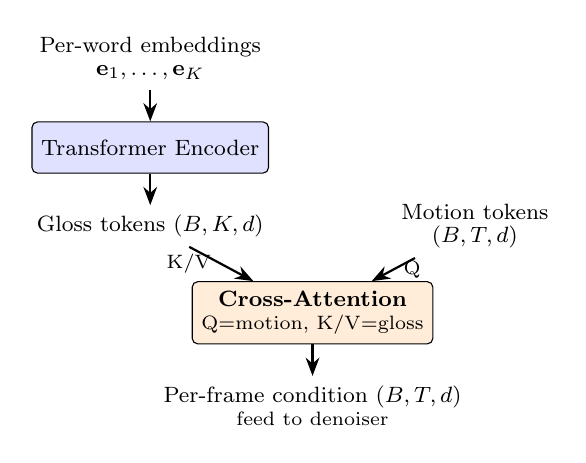
\begin{tikzpicture}[
    >=Stealth,
    node distance=0.5cm,
    box/.style={draw, rounded corners=2pt, minimum height=0.65cm, align=center, font=\footnotesize, minimum width=2.4cm},
    learned/.style={box, fill=blue!12},
    data/.style={font=\footnotesize, align=center},
    arrow/.style={->, thick},
]
\node[data] (input) {Per-word embeddings\\[-1pt]$\mathbf{e}_1, \ldots, \mathbf{e}_K$};
\node[learned, below=0.4cm of input] (enc) {Transformer Encoder};
\node[data, below=0.4cm of enc] (tokens) {Gloss tokens $(B, K, d)$};

\node[data, right=1.5cm of tokens] (motion) {Motion tokens\\[-1pt]$(B, T, d)$};

\node[learned, below=0.7cm of $(tokens)!0.5!(motion)$, fill=orange!15, minimum width=3.0cm] (xattn) {\textbf{Cross-Attention}\\[-1pt]{\scriptsize Q=motion, K/V=gloss}};

\node[data, below=0.4cm of xattn] (fused) {Per-frame condition $(B, T, d)$\\[-1pt]{\scriptsize feed to denoiser}};

\draw[arrow] (input) -- (enc);
\draw[arrow] (enc) -- (tokens);
\draw[arrow] (tokens) -- node[left, font=\scriptsize] {K/V} (xattn);
\draw[arrow] (motion) -- node[right, font=\scriptsize] {Q} (xattn);
\draw[arrow] (xattn) -- (fused);
\end{tikzpicture}
\caption{\textbf{VoteAlign}: Cross-attention attends from motion frames to gloss tokens, producing per-frame conditioning. No explicit gate needed.}
\label{fig:votealign}
\end{subfigure}
\caption{\textbf{Two learnable conditioning options compared in this work.}
(a)~\emph{VoteOnly}: a per-token sigmoid gate weights each gloss embedding, then mean-pools into a single global condition vector.
(b)~\emph{VoteAlign}: cross-attention produces \emph{per-frame} conditioning, where attention weights implicitly perform both token selection and temporal alignment, removing the need for an explicit gate. We report results for both as separate conditioning options under each denoiser variant.}
\label{fig:method_comparison}
\end{figure}

\subsection{Voting gate (VoteOnly)}
\label{sec:voting}

VoteOnly refines the LLM draft by assigning a learnable continuous keep/drop weight to each word, and pooling the gated representations into a single condition vector.

Each draft gloss word $g_k$ is independently embedded through the frozen text encoder (CLIP-ViT-B/32~\citep{radford2021clip} for How2Sign, XLM-RoBERTa-base~\citep{conneau2020xlmr} for PHOENIX-2014T), yielding per-word embeddings $\mathbf{e}_k \in \mathbb{R}^{d_\text{enc}}$.
Since the per-word embeddings are token-independent (each $\mathbf{e}_k$ is computed without seeing the other gloss words), we add a learnable positional encoding and pass the sequence through a lightweight trainable transformer encoder so that each output position can see every other position:
\begin{equation}
    \mathbf{h}_1, \ldots, \mathbf{h}_K = \text{TransEnc}(\mathbf{e}_1 + \mathbf{p}_1, \ldots, \mathbf{e}_K + \mathbf{p}_K)
\end{equation}
This is a vanilla pre-norm transformer encoder (PyTorch \texttt{nn.TransformerEncoder}) with no sign-language-specific structure; we use it solely to contextualize the otherwise independent per-word embeddings.
A linear head followed by sigmoid produces per-word gates:
\begin{equation}
    \alpha_k = \sigma(\mathbf{w}^\top \mathbf{h}_k + b), \quad \alpha_k \in [0, 1]
\end{equation}
The gate bias is initialized to $+1$ so that $\sigma(1) \approx 0.73$, biasing toward keeping words initially.
The gated representations are pooled into a single condition vector:
\begin{equation}
    \mathbf{c} = \text{MLP}\!\left(\frac{\sum_k \alpha_k \cdot \text{Proj}(\mathbf{h}_k)}{\sum_k \alpha_k}\right) \in \mathbb{R}^{d_\text{model}}
\end{equation}
This vector is prepended as a condition token to the denoiser, following standard practice~\citep{tevet2023human}.
The voting gate is trained end-to-end through the diffusion loss with no gloss-level supervision.

\subsection{Cross-attention temporal fusion (VoteAlign)}
\label{sec:fusion}

VoteOnly collapses all gloss information into a single vector, losing token-level temporal structure.
Sign languages use different word orders than their surrounding spoken languages (e.g., topic-comment structure in ASL), and different glosses correspond to different temporal segments of the motion.
Rather than explicitly reordering pseudo-glosses---which requires either heuristic algorithms~\citep{wong2025pgg} or separate training with video supervision---VoteAlign lets the model learn temporal alignment implicitly through cross-attention.

VoteAlign replaces the voting gate and mean pooling with a cross-attention fusion decoder (Figure~\ref{fig:votealign}).
The same trainable transformer encoder as in VoteOnly contextualizes the per-word embeddings (without the sigmoid gate), producing gloss tokens $\mathbf{h}_k \in \mathbb{R}^{d_\text{model}}$.
The noisy motion features $\mathbf{x}_t$ are projected and combined with positional encoding:
\begin{equation}
    \mathbf{m}_1, \ldots, \mathbf{m}_T = \text{PoseProj}(\mathbf{x}_t) + \text{PE}
\end{equation}
A transformer decoder performs cross-attention where motion tokens are \emph{queries} and gloss tokens are \emph{keys/values}:
\begin{equation}
    \mathbf{f}_1, \ldots, \mathbf{f}_T = \text{FusionDec}(\underbrace{\mathbf{m}_1, \ldots, \mathbf{m}_T}_{\text{query (motion)}}, \underbrace{\mathbf{h}_1, \ldots, \mathbf{h}_K}_{\text{key/value (gloss)}})
\end{equation}
The cross-attention weights $A_{t,k} = \text{softmax}(\mathbf{q}_t \mathbf{k}_k^\top / \sqrt{d})$ jointly encode two functions:
(1)~\textbf{selection}---irrelevant gloss tokens receive near-zero attention weight, and
(2)~\textbf{temporal alignment}---different frames attend to different gloss tokens, implicitly learning sign-language word order.
The fused features $\mathbf{f}_t$ are then processed by the main transformer encoder denoiser.

This design subsumes the explicit voting gate: attention weights naturally perform soft token selection (making a separate sigmoid gate unnecessary) while simultaneously learning temporal alignment.
The result is \emph{per-frame} conditioning rather than a single global vector, enabling temporally-varying control critical for sequential sign production.

\subsection{Phonological attribute conditioning}
\label{sec:phonology}

Pseudo-glosses capture \emph{which} signs to produce, but not \emph{how} to produce them.
Sign languages encode meaning through phonological parameters such as handshape, location, movement, and orientation~\citep{stokoe1960sign,brentari1998prosodic}, which are systematic across signers but not recoverable from gloss text alone.

\paragraph{Attribute extraction.}
We augment each LLM-drafted gloss token with phonological attributes from ASL-SignBank, a curated lexical database with per-sign phonological annotations. For each draft gloss word $g_k$ we look up its SignBank entry and extract a six-attribute categorical vector
\[
\mathbf{a}_k = \big(a_k^{\text{loc-maj}},\; a_k^{\text{loc-min}},\; a_k^{\text{fingers}},\; a_k^{\text{flexion}},\; a_k^{\text{nd-hs}},\; a_k^{\text{path}}\big),
\]
encoding two location features (major and minor), three handshape-related features (selected fingers, flexion, non-dominant handshape), and path movement. Lookup uses lemma matching combined with a keyword fallback (e.g., compound and morphological variants); the keyword fallback raises per-token training-set coverage from $16.7\%$ (lemma-only) to $86.7\%$. Tokens without a SignBank match are routed to a learned \emph{null} attribute embedding so that $\mathbf{a}_k$ is always defined.

\paragraph{Fusion with the gloss representation.}
Each categorical attribute is embedded through its own learned table; the six embeddings are concatenated and projected to a $d_{\text{phono}}{=}64$-dimensional phono token $\boldsymbol{\phi}_k$. We then concatenate $\boldsymbol{\phi}_k$ with the per-token gloss representation $\mathbf{u}_k$ at the fusion stage and project through a linear layer to obtain the augmented per-token representation:
\begin{equation}
    \mathbf{u}_k' = W_{\text{gp}} \cdot [\mathbf{u}_k \,;\, \boldsymbol{\phi}_k] + b_{\text{gp}}.
\end{equation}
The fusion stage differs by conditioning module to keep each module's downstream interface unchanged: under CFG, $\mathbf{u}_k = \mathbf{e}_k$ is the raw per-word embedding (fused before mean pooling, since CFG has no trainable transformer encoder over the tokens); under VoteOnly and VoteAlign, $\mathbf{u}_k = \mathbf{h}_k$ is the per-token output of the transformer encoder (fused before the sigmoid gate or the cross-attention decoder, respectively). In all three cases phonological augmentation is independent of and composable with the conditioning choice.

\paragraph{Empirical effect.}
Phonological augmentation provides our largest single FID\textsubscript{AE} improvement: on the kin denoiser with LLM-drafted gloss + VoteOnly, adding phono attributes reduces FID from $1.99$ to $1.94$ and FID\textsubscript{AE} from $5.55$ to $1.19$, a $4.7\times$ reduction in autoencoder-feature distance (Table~\ref{tab:main_results}). On the ms denoiser the effect is direction-mixed, suggesting non-trivial interaction between phono attributes and the multi-scale temporal pyramid. PHOENIX-2014T uses German Sign Language (DGS) and is not aligned to ASL-SignBank; we therefore report phonological-attribute conditioning only for How2Sign.

%=====================================================================
\section{Experiments}
\label{sec:experiments}

\subsection{Setup}
\label{sec:setup}

\paragraph{Datasets and filtering.}
We evaluate on two corpora: \textbf{How2Sign}~\citep{duarte2021how2sign} (American Sign Language, English; SMPL-X body fits from~\citep{hong2026phonologyguided}) and \textbf{PHOENIX-2014T}~\citep{camgoz2018neural} (German Sign Language, German; 2D upper-body MediaPipe joints, 67 keypoints, $D = 201$).
For How2Sign, we restrict to sentences of 3--30 words (median 15) to remove single-word fragments and a long tail of multi-sentence captions, yielding $26{,}070$ train / $1{,}954$ test sentences (a $\sim$16\% reduction; the largest cause is sentences longer than 30 words).
PHOENIX-2014T sentences are naturally short (median 7 words) and require no length filtering; we use $7{,}004$ train / $634$ test, after dropping a small number of clips with missing pose extractions.
All motion sequences are padded or uniformly subsampled to a fixed length: $T=100$ frames for How2Sign and $T=160$ for PHOENIX-2014T (chosen to match the typical signing duration of each corpus while keeping batches uniform).

\paragraph{Metrics.}
We report five primary metrics in main-paper tables: \emph{FID} (frame-statistic Fr\'echet distance, computed on raw motion features); \emph{FID\textsubscript{AE}} (Fr\'echet distance in the bottleneck space of a self-trained motion autoencoder, defined below); \emph{F\textsubscript{lh}} and \emph{F\textsubscript{rh}} (region-specific FID restricted to the left- and right-hand joints, capturing manual articulation quality); and \emph{JerkR}, the ratio of generated to ground-truth third-derivative magnitude (perfect = $1$; values $\not\in [0.3, 5]$ flag degenerate motion---near-deterministic autoregressive output below $0.3$, runaway jitter above $5$).
We additionally report BLEU-1 and R@10 computed by back-translating generated motion to spoken-language text via a self-trained back-translation model (Section~\ref{sec:eval_models}). We deliberately omit BLEU-2/3/4: our pseudo-gloss conditioning treats glosses as a per-token bag rather than a connected phrase, and sign languages systematically reorder content relative to spoken English (e.g., topic-comment), so n-gram precision metrics penalize legitimate reorderings that the bag-of-glosses input does not constrain. BLEU-1 measures unigram (semantic content) overlap, which is what the gloss-to-motion pipeline is designed to preserve.
Full-sweep tables (Tables~\ref{tab:h2s_full},~\ref{tab:phoenix_full}) report every checkpoint we trained under the unified protocol; main-paper tables present a curated subset for readability.

\paragraph{Self-trained evaluation models.}
\label{sec:eval_models}
Two metrics in our tables---FID\textsubscript{AE} and back-translation BLEU/R@k---require auxiliary models that are not publicly released for sign-language motion under our preprocessing. We train both ourselves and treat them as \emph{relative rankers} among methods evaluated under identical conditions, rather than absolute fidelity scores.

\textbf{Motion autoencoder for FID\textsubscript{AE}.} We train a transformer-based motion autoencoder (encoder/decoder, fixed-length input matching the dataset's $T$, joint-region weighted reconstruction loss matching our generation loss) on the corresponding training split, and compute FID\textsubscript{AE} in the encoder's bottleneck feature space. We find FID\textsubscript{AE} more sensitive to motion-distribution differences than per-frame statistic FID, particularly for diagnosing autoregressive mode collapse where raw FID can appear competitive while motion is near-deterministic (Section~\ref{sec:results}). The autoencoder is itself learned and not perfect, so small FID\textsubscript{AE} differences should not be over-interpreted; we use it for ranking and for the FID-vs-FID\textsubscript{AE} divergence diagnostic.

\textbf{Back-translation model for BLEU-1/R@k.} Following~\citet{baltatzis2024neural}, we report BLEU and R@k computed by back-translating generated motion to spoken-language text. No public BT model is released for either dataset under our preprocessing, so we train our own transformer encoder--decoder with a 10K-word vocabulary; we use beam-search decoding (beam=5) for BLEU-1 and length-normalized log-probability ranking against 99 distractors for R@k. As a ceiling, decoding ground-truth motion through our BT model yields BLEU-1 = 15.54 on How2Sign and 13.20 on PHOENIX-2014T (Tables~\ref{tab:h2s_full},~\ref{tab:phoenix_full}); these are upper bounds for any generated-motion row in our tables. BT models trained on tens of thousands of (motion, text) pairs cannot reach the BLEU levels of large-scale spoken-language MT, so we treat BT-BLEU-1 as a relative comparison signal rather than an absolute fidelity metric, and caution against cross-protocol comparison of absolute values.

\paragraph{Within-paper consistency.}
Sign-language production has historically reported metrics under heterogeneous and often unspecified evaluation protocols (frame rate, joint subset, sentence-length filtering, FID feature extractor), making cross-paper comparisons unreliable. We deliberately depart from this practice: (i) we re-implement all baselines, including Progressive Transformers~\citep{saunders2020progressive} and Neural Sign Actors~\citep{baltatzis2024neural}, in our codebase; (ii) we train and evaluate \emph{all} compared methods---ours and baselines---on identical filtered splits, identical sequence lengths, identical text encoders, and the same self-trained FID\textsubscript{AE} and BT models; and (iii) we do not cite numbers from prior works directly, even when their setting is nominally similar, because subtle differences can shift FID by a factor of two or more. All in-paper rankings therefore reflect method quality rather than evaluation differences. Researchers wishing to recover other papers' protocols can apply our public code to the unmodified test split.

\paragraph{Implementation details.}
All diffusion models use the same MDM-style framework: $4$-layer transformer-encoder denoiser, $d_{\text{model}}=512$, $8$ attention heads, cosine noise schedule with $T=1000$ training steps, DDIM sampling with $50$ inference steps, $\epsilon$-prediction, CFG with unconditional probability $0.1$ and guidance scale $w=3.0$. Text conditioning uses CLIP-ViT-B/32 (How2Sign) or XLM-RoBERTa-base (PHOENIX-2014T; we shorthand it ``mclip'' for the multilingual conditioning role, but it is not a multilingual CLIP variant), both frozen. LLM-drafted pseudo-glosses are pre-computed once with Qwen2.5-32B-Instruct running locally and cached to disk. Training uses AdamW with learning rate $10^{-4}$ cosine-annealed to $10^{-6}$, batch size $64$, for $100$ epochs on a single NVIDIA A100 (20GB MIG partition). For each run we save three checkpoints---\emph{best} (lowest training loss), \emph{second-best}, and \emph{newest}---and report metrics from \texttt{best\_model.pt} only. The trainable transformer encoder over the gloss tokens (used by both VoteOnly and VoteAlign) has $2$ layers with $4$ heads; the gate itself is a single linear head followed by sigmoid. The cross-attention fusion decoder of VoteAlign has $2$ layers with $8$ heads. Phonological-attribute conditioning uses $6$ SignBank attributes (major and minor location, selected fingers, flexion, non-dominant handshape, and path movement) embedded into a $64$-dimensional phono token, fused per-position with the gloss embedding before the voting gate (VoteOnly) or cross-attention decoder (VoteAlign). Full hyperparameter tables and per-method ablation budgets are in Appendix~\ref{app:details}.

\subsection{Conditioning ablation}
\label{sec:ablation}

We compare the six conditioning strategies introduced in Section~\ref{sec:method} below, all using the same base diffusion architecture:

\begin{table}[t]
  \caption{\textbf{Main How2Sign results, filtered+seq100 protocol} (1,954 test sentences, seed=42). All diffusion models use the V1 architecture with $\epsilon$-prediction and CFG ($w=3.0$). Denoisers (MDM, ms = multi-scale, kin = temporal bias) are defined in Section~\ref{sec:backbones}. Best in \textbf{bold}; the H2S champion is starred. $\downarrow$: lower is better; $\uparrow$: higher is better. JerkR is the ratio of generated to ground-truth jerk (closer to 1 is better; values $\notin [0.3, 5]$ indicate degenerate motion). Full 20-row results in Table~\ref{tab:h2s_full}.}
  \label{tab:main_results}
  \centering
  \small
  \begin{tabular}{llcccccc}
    \toprule
    \textbf{Method} & \textbf{Input} & \textbf{FID}$\downarrow$ & \textbf{FID\textsubscript{AE}}$\downarrow$ & \textbf{F\textsubscript{lh}}$\downarrow$ & \textbf{F\textsubscript{rh}}$\downarrow$ & \textbf{JerkR} & \textbf{B-1}$\uparrow$ \\
    \midrule
    \multicolumn{8}{l}{\textit{Prior baselines}} \\
    \quad Progressive Transformers & sent & 3.30           & ---           & ---           & ---           & 0.02 $\,$\textsuperscript{$\dagger$} & \placeholder{TBD} \\
    \quad Neural Sign Actors       & sent & 151.61         & 757.0         & ---           & ---           & ---  & \placeholder{TBD} \\
    \midrule
    \multicolumn{8}{l}{\textit{Sentence-only diffusion baseline}} \\
    \quad MDM $\cdot$ CFG                                          & sent           & 2.24          & 4.13          & 0.12          & 0.14          & 1.31          & \placeholder{TBD} \\
    \midrule
    \multicolumn{8}{l}{\textit{Pseudo-gloss conditioning}} \\
    \quad ms  $\cdot$ VoteAlign                                    & rule           & 2.13          & 3.51          & 0.08          & 0.08          & 1.12          & \placeholder{TBD} \\
    \quad ms  $\cdot$ VoteOnly                                     & LLM            & 2.15          & \textbf{0.74} & 0.09          & 0.18          & 1.09          & \placeholder{TBD} \\
    \quad ms  $\cdot$ VoteOnly                                     & LLM+phono      & 2.03          & 3.36          & 0.08          & \textbf{0.03} & \textbf{1.05} & \placeholder{TBD} \\
    \quad kin $\cdot$ VoteOnly                                     & LLM            & 1.99          & 5.55          & 0.09          & \textbf{0.04} & 1.23          & \placeholder{TBD} \\
    \quad \textbf{kin $\cdot$ VoteOnly} $\bigstar$                 & LLM+phono      & \textbf{1.94} & 1.19          & \textbf{0.07} & 0.05          & 1.36          & \placeholder{TBD} \\
    \bottomrule
  \end{tabular}
  \par\smallskip
  \footnotesize $^\dagger$ JerkR $\ll 0.3$ indicates near-deterministic autoregressive output (mode collapse).
\end{table}

\begin{table}[t]
  \caption{\textbf{Main PHOENIX-2014T results, mclip text encoder} (634 test sentences, seed=42). Same denoisers and conditioning architectures as Table~\ref{tab:main_results}; phonological-attribute conditioning is omitted because PHOENIX-2014T does not release SignBank-aligned signs, and we instead include ground-truth gloss as a Phoenix-specific input. Best in \textbf{bold}; the Phoenix champion (best FID\textsubscript{AE}) is starred. Full 20-row results in Table~\ref{tab:phoenix_full}.}
  \label{tab:phoenix_main}
  \centering
  \small
  \begin{tabular}{llcccccc}
    \toprule
    \textbf{Method} & \textbf{Input} & \textbf{FID}$\downarrow$ & \textbf{FID\textsubscript{AE}}$\downarrow$ & \textbf{F\textsubscript{lh}}$\downarrow$ & \textbf{F\textsubscript{rh}}$\downarrow$ & \textbf{JerkR} & \textbf{B-1}$\uparrow$ \\
    \midrule
    \multicolumn{8}{l}{\textit{Prior baselines}} \\
    \quad Progressive Transformers & sent & 16.64           & ---           & ---           & ---           & 0.09 $\,$\textsuperscript{$\dagger$} & \textbf{8.80} \\
    \quad Neural Sign Actors       & sent & 180.14          & 232.21        & 16.56         & 25.13         & 62.4 $\,$\textsuperscript{$\dagger$} & --- \\
    \midrule
    \multicolumn{8}{l}{\textit{Sentence input (single representative; $\cdot$ms / $\cdot$kin appear in Table~\ref{tab:phoenix_full})}} \\
    \quad MDM $\cdot$ CFG                                          & sent           & 33.17          & 19.43         & 7.46          & 8.93          & 4.59          & 6.48 \\
    \midrule
    \multicolumn{8}{l}{\textit{Pseudo-gloss / GT-gloss conditioning}} \\
    \quad ms $\cdot$ Voting                                        & LLM            & 23.88          & 10.12         & \textbf{1.91} & 5.54          & 3.11          & 6.11 \\
    \quad \textbf{ms $\cdot$ Voting} $\bigstar$                    & gt             & 21.81          & \textbf{6.28} & 4.68          & 1.53          & 2.71          & 7.18 \\
    \quad kin $\cdot$ VoteAlign                                    & rule           & 35.49          & 12.61         & 7.23          & 6.82          & 2.19          & 5.84 \\
    \quad kin $\cdot$ Voting                                       & LLM            & 28.36          & 9.44          & 4.04          & \textbf{0.94} & 2.42          & 6.80 \\
    \quad kin $\cdot$ Voting                                       & gt             & 31.62          & 9.92          & 2.28          & 4.29          & 3.55          & 7.22 \\
    \bottomrule
  \end{tabular}
  \par\smallskip
  \footnotesize $^\dagger$ JerkR far from 1 indicates degenerate motion (collapse for PT; runaway jitter for NSA).
\end{table}

\paragraph{Sentence conditioning.}
The full sentence is encoded by the frozen text encoder into a single embedding vector, projected through a 3-layer MLP, and prepended as a condition token to the denoiser.
This is the standard approach in text-to-motion models~\citep{tevet2023human,hong2026phonologyguided}.

\paragraph{Rule-based gloss conditioning.}
We extract pseudo-glosses using hand-crafted linguistic rules: POS filtering (keep nouns, verbs, adjectives, adverbs), lemmatization with ASL-specific handling (preserve pronouns and negations, normalize contractions, drop discourse markers), following \citet{hong2026phonologyguided}.
The gloss string is encoded by the frozen text encoder through a separate 3-layer MLP.

\paragraph{LLM-drafted gloss conditioning.}
Same architecture as rule-based, but using LLM-extracted pseudo-glosses (Section~\ref{sec:draft}).

\paragraph{Per-token vs whole-string gloss encoding.}
We encode each pseudo-gloss token independently through CLIP and mean-pool the resulting embeddings, rather than concatenating the gloss list into a single string before encoding.
Per-token encoding preserves token-level structure that is later required by the voting gate (Section~\ref{sec:voting}) and the cross-attention fusion (Section~\ref{sec:fusion}); whole-string encoding collapses the gloss list to a single CLIP sentence-level embedding, discarding token boundaries.
Table~\ref{tab:gloss_encoding_ablation} reports an ablation on the simplest CFG conditioning, where both encodings produce the same downstream interface, isolating the effect of the encoding granularity itself. Per-token wins on FID\textsubscript{AE} on both gloss sources (rule: 2.34 vs 3.03, $-23\%$; LLM: 1.58 vs 3.02, $-48\%$) and on raw FID with LLM gloss (2.03 vs 2.10); whole-string only edges per-token by $0.18$ FID on the lower-quality rule gloss, while losing the same row on FID\textsubscript{AE} by $0.69$. We therefore adopt per-token encoding throughout, both for the consistent FID\textsubscript{AE} advantage and because it is required by the voting and fusion modules below.

\begin{table}[h]
  \caption{\textbf{Pseudo-gloss encoding ablation on How2Sign} (MDM denoiser, CFG conditioning, $w=3.0$). Per-token encoding (each gloss word independently embedded then mean-pooled) vs whole-string encoding (joined gloss list embedded as a single CLIP input); lower is better. Per-token wins FID\textsubscript{AE} on both gloss sources; whole-string only edges per-token on raw FID under the lower-quality rule gloss.}
  \label{tab:gloss_encoding_ablation}
  \centering
  \small
  \begin{tabular}{llcc}
    \toprule
    \textbf{Encoding} & \textbf{Gloss src} & \textbf{FID}$\downarrow$ & \textbf{FID\textsubscript{AE}}$\downarrow$ \\
    \midrule
    per-token    & rule        & 2.23          & 2.34          \\
    whole-string & rule        & 2.05          & 3.03          \\
    per-token    & LLM-drafted & \textbf{2.03} & \textbf{1.58} \\
    whole-string & LLM-drafted & 2.10          & 3.02          \\
    \bottomrule
  \end{tabular}
\end{table}

\paragraph{VoteOnly (ours).}
Per-word embedding $\to$ trainable transformer encoder $\to$ sigmoid gate $\to$ weighted mean pool $\to$ single condition vector (Section~\ref{sec:voting}).

\paragraph{VoteAlign (ours).}
Trainable transformer encoder + cross-attention fusion (Section~\ref{sec:fusion}).
Instead of collapsing gloss tokens into a single vector, the fusion decoder produces per-frame conditioning via cross-attention, learning both selection and temporal alignment.

\subsection{Results}
\label{sec:results}

\placeholder{
Discussion of Tables~\ref{tab:main_results} and~\ref{tab:phoenix_main} to be written. Anchor points (numbers verified, just need prose):
\begin{itemize}
  \item How2Sign champion = kin-VoteOnly with LLM+phono input (FID \textbf{1.94} / FID\textsubscript{AE} \textbf{1.19}). Phono delta on kin: FID 1.99$\to$1.94, FID\textsubscript{AE} 5.55$\to$1.19 (4.7$\times$). Phono on ms is direction-mixed.
  \item PHOENIX-2014T headline = ms-Voting with gt gloss (FID \textbf{21.81} / FID\textsubscript{AE} \textbf{6.28}); next best = ms-Voting with LLM gloss (23.88 / 10.12).
  \item Pseudo-gloss + voting beats sentence-only MDM on both datasets.
  \item VoteAlign underperforms VoteOnly under our protocol; on PHOENIX it is even worse than MDM-CFG-sent baseline.
  \item Prior baselines collapse: PT-SMPL-X JerkR 0.02 (autoregressive mode collapse); NSA fails to converge (FID 151.6 / 180.1) under our re-implementation.
  \item FID vs FID\textsubscript{AE} divergence is itself a useful diagnostic; refer to Tables~\ref{tab:h2s_full} and~\ref{tab:phoenix_full} for the full sweep.
\end{itemize}
}

\subsection{Analysis}
\label{sec:analysis}

\placeholder{Analysis subsection to be written.}

\paragraph{What does VoteAlign learn? Cross-attention alignment patterns.}

\begin{figure}[t]
    \centering
    \fbox{\rule[-.5cm]{0cm}{4cm} \rule[-.5cm]{13cm}{0cm}}
    \caption{\textbf{Cross-attention alignment patterns in VoteAlign.}
    \placeholder{Visualization of attention weights $A_{t,k}$ from the VoteAlign decoder for example sentences, showing how different gloss tokens dominate different temporal segments of the generated motion. Even when VoteAlign does not win on FID, examining its attention provides a window into the gloss--motion mapping.}}
    \label{fig:attention}
\end{figure}

\placeholder{Figure~\ref{fig:attention} visualizes the cross-attention weights between motion frames (queries) and gloss tokens (keys/values) from a trained VoteAlign model. The attention patterns show clear temporal structure: different gloss words dominate different temporal segments, and the ordering of attended segments does not always follow the spoken-language word order, suggesting that VoteAlign learns a soft gloss-to-motion temporal mapping during training.}

\paragraph{Quantitative alignment evaluation.}
\placeholder{To quantify whether VoteAlign's cross-attention learns meaningful temporal alignment rather than diffuse attention, we extract the dominant gloss for each frame (argmax over attention weights) and compare the resulting gloss ordering against GT gloss timing derived from forced alignment.
We report: (1) Kendall's $\tau$ rank correlation between predicted and GT gloss order, and (2) segment-boundary F1 (whether attention transitions align with GT sign boundaries).
Results: $\tau = $ X.XX, boundary F1 = X.XX, against a spoken-language-order baseline of $\tau = $ X.XX. We caveat that the alignment-quality story does not by itself rescue VoteAlign's overall ranking on FID and FID\textsubscript{AE}; we report it for diagnostic value rather than as a competitive advantage.}

\subsection{Qualitative results}

\begin{figure}[t]
    \centering
    \fbox{\rule[-.5cm]{0cm}{5cm} \rule[-.5cm]{13cm}{0cm}}
    \caption{\textbf{Qualitative comparison.}
    \placeholder{Rendered SMPL-X meshes for example sentences comparing GT motion, MDM-CFG (sent), kin-VoteOnly (LLM+phono), and ms-VoteOnly (LLM). Highlight handshape accuracy on signs covered by SignBank (where phono helps) and temporal alignment on multi-sign phrases.}}
    \label{fig:qualitative}
\end{figure}


%=====================================================================
\section{Discussion and Limitations}
\label{sec:discussion}

\paragraph{Cross-attention subsumes explicit gating.}
A key finding is that cross-attention naturally performs token selection via attention weights, making an explicit sigmoid gate unnecessary.
In preliminary experiments with a combined gate + cross-attention architecture, the gate collapsed to zero (all tokens suppressed) while the cross-attention module compensated through its residual connection.
Removing the gate and relying solely on cross-attention for both selection and alignment yielded a cleaner architecture with better gradient flow.

\paragraph{Limitations.}
Our approach has several limitations.
First, the LLM draft quality is bounded by the few-shot examples and the LLM's understanding of sign language linguistics.
Second, the cross-attention alignment is implicit and soft, which may be insufficient for capturing hard temporal boundaries between signs.
Third, phonological attribute coverage depends on SignBank's vocabulary; glosses absent from SignBank fall back to text-only conditioning.
Fourth, our evaluation relies on distribution-level metrics (FID) and per-joint error (MPJPE); perceptual evaluation by sign language users would provide stronger validation.


%=====================================================================
\section{Conclusion}
\label{sec:conclusion}

We presented a systematic study of two complementary design axes for diffusion-based sign language production: \emph{conditioning input} (sentence, rule-based and LLM-drafted pseudo-gloss, token-level voting, cross-attention fusion, and SignBank phonological attributes) and \emph{denoiser architecture} (the temporal-bias variant kin and the multi-scale variant ms, both extending the MDM transformer-encoder denoiser). Across How2Sign and PHOENIX-2014T, we find that the optimal combination is dataset-dependent rather than universal: kin with LLM-drafted gloss + token voting + phonological attributes wins on How2Sign, while ms with token voting on ground-truth gloss wins on PHOENIX-2014T. Under our unified evaluation protocol, simpler token-level voting consistently dominates the more complex per-frame cross-attention fusion, and prior baselines do not survive controlled re-implementation. We release all code, splits, evaluation pipelines, and trained checkpoints.
\placeholder{Future work: perceptual evaluation by sign-language users; extension to additional sign languages; signed-language-specific motion-AE pretraining; integration of NMS (non-manual signal) channels such as facial expression and body posture into the conditioning.}


%=====================================================================
\begin{ack}
\placeholder{Acknowledgments will be added in the camera-ready version.}
\end{ack}

%=====================================================================
\bibliographystyle{plainnat}

\begin{thebibliography}{30}

\bibitem[Bahdanau et al.(2015)]{bahdanau2015neural}
Dzmitry Bahdanau, Kyunghyun Cho, and Yoshua Bengio.
\newblock Neural machine translation by jointly learning to align and translate.
\newblock In \emph{ICLR}, 2015.

\bibitem[Brentari(1998)]{brentari1998prosodic}
Diane Brentari.
\newblock \emph{A Prosodic Model of Sign Language Phonology}.
\newblock MIT Press, 1998.

\bibitem[Chen et al.(2023)]{chen2023mld}
Xin Chen, Biao Jiang, Wen Liu, Zilong Huang, Bin Fu, Tao Chen, and Gang Yu.
\newblock Executing your commands via motion diffusion in latent space.
\newblock In \emph{CVPR}, 2023.

\bibitem[Conneau et al.(2020)]{conneau2020xlmr}
Alexis Conneau, Kartikay Khandelwal, Naman Goyal, Vishrav Chaudhary, Guillaume Wenzek, Francisco Guzm{\'a}n, Edouard Grave, Myle Ott, Luke Zettlemoyer, and Veselin Stoyanov.
\newblock Unsupervised cross-lingual representation learning at scale.
\newblock In \emph{ACL}, 2020.

\bibitem[Cox et al.(2002)]{cox2002tessa}
Stephen Cox, Michael Lincoln, Judy Tryggvason, Melanie Nakisa, Mark Wells, Marcus Tutt, and Sanja Abbott.
\newblock {TESSA}, a system to aid communication with deaf people.
\newblock In \emph{ASSETS}, 2002.

\bibitem[Baltatzis et al.(2024)]{baltatzis2024neural}
Vasileios Baltatzis, Rolandos~Alexandros Potamias, Evangelos Ververas, Guanxiong Sun, Jiankang Deng, and Stefanos Zafeiriou.
\newblock Neural sign actors: A diffusion model for {3D} sign language production from text.
\newblock In \emph{CVPR}, 2024.

\bibitem[Duarte et al.(2021)]{duarte2021how2sign}
Amanda Duarte, Shruti Palaskar, Lucas Ventura, Deepti Ghadiyaram, Kenneth DeHaan, Florian Metze, Jordi Torres, and Xavier Gir{\'o}-i-Nieto.
\newblock How2sign: A large-scale multimodal dataset for continuous {A}merican {S}ign {L}anguage.
\newblock In \emph{CVPR}, 2021.

\bibitem[Fang et al.(2023)]{fang2023signdiff}
Yuanzhi Fang, Mitsuru Nakazawa, Yun-Chang Huang, and Shuji Kosugi.
\newblock SignDiff: Learning diffusion models for {A}merican sign language production.
\newblock \emph{arXiv preprint arXiv:2308.16082}, 2023.

\bibitem[Ho and Salimans(2022)]{ho2022classifier}
Jonathan Ho and Tim Salimans.
\newblock Classifier-free diffusion guidance.
\newblock In \emph{NeurIPS Workshop on Deep Generative Models and Downstream Applications}, 2022.

\bibitem[Hong and Kosecka(2026)]{hong2026phonologyguided}
Rui Hong and Jana Kosecka.
\newblock Toward phonology-guided sign language motion generation: A diffusion baseline and conditioning analysis.
\newblock \emph{arXiv preprint arXiv:2603.17388}, 2026.

\bibitem[McDonald et al.(2016)]{mcdonald2016automated}
John McDonald, Rosalee Wolfe, Jerry Schnepp, Julie Hochgesang, Diana Gorman Jamrozik, Marie Stumbo, Larwan Berke, Melissa Bialek, and Farah Thomas.
\newblock An automated technique for real-time production of lifelike animations of {A}merican {S}ign {L}anguage.
\newblock \emph{Universal Access in the Information Society}, 15(4):551--566, 2016.

\bibitem[Radford et al.(2021)]{radford2021clip}
Alec Radford, Jong~Wook Kim, Chris Hallacy, Aditya Ramesh, Gabriel Goh, Sandhini Agarwal, Girish Sastry, Amanda Askell, Pamela Mishkin, Jack Clark, et~al.
\newblock Learning transferable visual models from natural language supervision.
\newblock In \emph{ICML}, 2021.

\bibitem[Sandler and Lillo-Martin(2006)]{sandler2006sign}
Wendy Sandler and Diane Lillo-Martin.
\newblock \emph{Sign Language and Linguistic Universals}.
\newblock Cambridge University Press, 2006.

\bibitem[Saunders et al.(2020)]{saunders2020progressive}
Ben Saunders, Necati~Cihan Bolge, and Richard Sherfield.
\newblock Progressive transformers for end-to-end sign language production.
\newblock In \emph{ECCV}, 2020.

\bibitem[Saunders et al.(2021)]{saunders2021continuous}
Ben Saunders, Necati~Cihan Bolge, and Richard Sherfield.
\newblock Continuous {3D} multi-channel sign language production via progressive transformers and mixture density networks.
\newblock \emph{IJCV}, 129(7):2113--2130, 2021.

\bibitem[Song et al.(2021)]{song2021denoising}
Jiaming Song, Chenlin Meng, and Stefano Ermon.
\newblock Denoising diffusion implicit models.
\newblock In \emph{ICLR}, 2021.

\bibitem[Stokoe(1960)]{stokoe1960sign}
William~C. Stokoe.
\newblock Sign language structure: An outline of the visual communication systems of the {A}merican deaf.
\newblock \emph{Studies in Linguistics: Occasional Papers}, 8, 1960.

\bibitem[Tevet et al.(2023)]{tevet2023human}
Guy Tevet, Sigal Raab, Brian Gordon, Yonatan Shafir, Daniel Cohen-Or, and Amit~H. Bermano.
\newblock Human motion diffusion model.
\newblock In \emph{ICLR}, 2023.

\bibitem[Vaswani et al.(2017)]{vaswani2017attention}
Ashish Vaswani, Noam Shazeer, Niki Parmar, Jakob Uszkoreit, Llion Jones, Aidan~N. Gomez, \L{}ukasz Kaiser, and Illia Polosukhin.
\newblock Attention is all you need.
\newblock In \emph{NeurIPS}, 2017.

\bibitem[Walsh et al.(2024)]{walsh2024select}
Euan Walsh, Ben Saunders, and Richard Bowden.
\newblock Select and reorder: A novel approach for neural sign language production.
\newblock In \emph{LREC-COLING}, 2024.

\bibitem[Wong et al.(2025)]{wong2025pgg}
Ping~Lun Wong, Yijun~Jie Li, and Trevor Cohn.
\newblock Bridging sign and spoken languages: Pseudo gloss generation for sign language translation.
\newblock In \emph{NeurIPS}, 2025.

\bibitem[Xie et al.(2024)]{xie2024t2sgpt}
Pan Xie, Qipeng Zhang, Tong Li, Jianqiang Huang, Xuemei Wang, and Zheng Wang.
\newblock {T2S-GPT}: Dynamic vector quantization for autoregressive sign language production from text.
\newblock In \emph{ACL}, 2024.

\bibitem[Zhang et al.(2022)]{zhang2022motiondiffuse}
Mingyuan Zhang, Zhongang Cai, Liang Pan, Fangzhou Hong, Xinying Guo, Lei Yang, and Ziwei Liu.
\newblock {MotionDiffuse}: Text-driven human motion generation with diffusion model.
\newblock \emph{arXiv preprint arXiv:2208.15001}, 2022.

\bibitem[Zheng et al.(2023)]{zheng2023sign2gpt}
Benjamin Zheng, Biao Zhang, Jinsong Su, Yidong Chen, and Jiajun Zhang.
\newblock Sign2{GPT}: Leveraging large language models for gloss-free sign language translation.
\newblock In \emph{ICLR}, 2024.

\bibitem[Azadi et al.(2024)]{azadi2024make}
Samaneh Azadi, Akbar Shah, Thomas Hayes, Devi Parikh, and Sonal Gupta.
\newblock Make-an-animation: Large-scale text-conditional {3D} human motion generation.
\newblock In \emph{ICCV}, 2024.

\bibitem[Petrovich et al.(2022)]{petrovich2022temos}
Mathis Petrovich, Michael~J. Black, and G{\"u}l Varol.
\newblock {TEMOS}: Generating diverse human motions from textual descriptions.
\newblock In \emph{ECCV}, 2022.

\bibitem[Camg{\"o}z et al.(2018)]{camgoz2018neural}
Necati~Cihan Camg{\"o}z, Simon Hadfield, Oscar Koller, Hermann Ney, and Richard Bowden.
\newblock Neural sign language translation.
\newblock In \emph{CVPR}, 2018.

\end{thebibliography}

%%%%%%%%%%%%%%%%%%%%%%%%%%%%%%%%%%%%%%%%%%%%%%%%%%%%%%%%%%%%

\appendix

\section{Additional experimental details}
\label{app:details}

\subsection{LLM prompt template}
\label{app:llm_prompt}

We use Qwen2.5-32B-Instruct with greedy decoding.
The system prompt assigns an ``ASL linguistic expert'' persona and instructs the model to follow the three-step procedure described in Section~\ref{sec:draft}.
The full prompt consists of:
\begin{enumerate}
    \item A role description and task definition: ``extract pseudo-gloss from an English sentence; each word should correspond to a distinct sign that an ASL signer would produce.''
    \item Detailed instructions for each of the three steps (phrase-level chunking, core meaning filtering, citation form restoration), including explicit lists of what to keep and drop.
    \item 31 hand-curated sentence--gloss example pairs covering diverse phenomena: auxiliary chains (``we're going to be learning'' $\to$ ``we learn''), light verb constructions (``take a look'' $\to$ ``look''), discourse markers (``let's do it slow'' $\to$ ``slow''), pronoun and negation preservation (``you don't have to take big steps'' $\to$ ``you not take big step''), phrasal verbs (``hold down the second string'' $\to$ ``hold down second string''), and degree modifier removal (``that's very challenging'' $\to$ ``challenging'').
    \item An output format instruction: ``Output ONLY the pseudo-gloss as a single line of space-separated lowercase words.''
\end{enumerate}

The sentence to be processed is appended after the examples as ``Sentence: \{input\}$\backslash$nGloss:'', and the first line of the LLM output is taken as the pseudo-gloss.
All results are cached to disk per split (train/val/test), so the LLM is invoked only once per sentence.

\subsection{Rule-based extraction rules}
\label{app:rule_details}

The rule-based baseline applies the following deterministic NLP pipeline using NLTK:

\begin{enumerate}
    \item \textbf{Tokenization and POS tagging.} NLTK \texttt{word\_tokenize} + \texttt{pos\_tag}.
    \item \textbf{Auxiliary bigram detection.} Multi-word auxiliary patterns are identified and dropped as a unit:
    \emph{(be-form)} + ``going'' + ``to'' + VB* $\to$ drop ``going'' (but keep ``going'' as a motion verb before nouns);
    \emph{(have-aux)} + ``got'' $\to$ drop ``got'';
    ``got'' + ``to'' + VB* $\to$ drop ``got''.
    \item \textbf{Content-word POS filter.} Keep tokens tagged as nouns (NN*), verbs (VB*), adjectives (JJ*), or adverbs (RB*).
    \item \textbf{Special-case preservation.} Pronouns (PRP, PRP\$), negations (\texttt{no, not, never, nothing, none, nobody}), and WH-words are explicitly kept regardless of POS tag. The contraction \texttt{n't} is normalized to \texttt{not}.
    \item \textbf{Lemmatization.} POS-gated irregular lookup tables (separate for verbs, adjectives, nouns) followed by rule-based suffix stripping with guards for natural doubled consonants and silent-e restoration.
    \item \textbf{ASL stopword removal.} Discourse markers (\texttt{so, therefore, however, just, actually, basically, literally}, etc.) are removed.
\end{enumerate}

\paragraph{Hyperparameter sensitivity.}
\placeholder{Ablation over transformer encoder depth (1 vs 2 vs 4 layers), fusion decoder depth (1 vs 2 vs 4 layers), guidance scale, and batch size.}

\section{Full results tables}
\label{app:full_tables}

This appendix provides the complete (un-condensed) result tables for both datasets.
Main-paper Tables present a curated subset for readability; the tables below report every checkpoint we trained under the unified evaluation protocol of Section~\ref{sec:experiments}.
\textbf{Method} = denoiser~$\cdot$~conditioning architecture (MDM = vanilla diffusion transformer; kin / vel / ms = temporal-bias, velocity-aware, multi-scale variants; CFG = single-vector conditioning; VoteOnly = token-gated mean pool; VoteAlign = cross-attention fusion).
\textbf{Input} = the conditioning signal fed to that method (\emph{sent} = English sentence only; \emph{rule} / \emph{LLM} / \emph{LLM-shuf} = pseudo-gloss source; \emph{gt} / \emph{trans} = ground-truth gloss / German translation for PHOENIX; suffixes \emph{+phono} and \emph{+pfx} indicate phonological-attribute conditioning and sentence prefix, respectively).
BLEU-1 column entries are placeholders to be filled by the back-translation evaluation; we report only BLEU-1 (unigram overlap) for the reasons given in Section~\ref{sec:setup}.

\begin{table}[h]
  \caption{\textbf{Full How2Sign results, filtered+seq100 protocol.} 20 ours/ablation checkpoints + Progressive Transformer~\citep{saunders2020progressive} + Neural Sign Actors~\citep{baltatzis2024neural} baselines. All numbers from the \texttt{best\_model.pt} checkpoint. JerkR is the ratio of generated to ground-truth jerk (closer to 1 is better; values $\notin [0.3, 5]$ indicate degenerate motion).}
  \label{tab:h2s_full}
  \centering
  \scriptsize
  \begin{tabular}{llcccccc}
    \toprule
    \textbf{Method} & \textbf{Input} & \textbf{FID}$\downarrow$ & \textbf{FID\textsubscript{AE}}$\downarrow$ & \textbf{F\textsubscript{lh}}$\downarrow$ & \textbf{F\textsubscript{rh}}$\downarrow$ & \textbf{JerkR} & \textbf{BLEU-1}$\uparrow$ \\
    \midrule
    kin $\cdot$ VoteOnly       & LLM-shuf       & \textbf{1.94} & 0.95          & 0.06          & 0.05          & 1.31 & \placeholder{TBD} \\
    kin $\cdot$ VoteOnly       & LLM+phono      & \textbf{1.94} & \textbf{1.19} & 0.07          & 0.05          & 1.36 & \placeholder{TBD} \\
    ms $\cdot$ VoteOnly        & LLM-shuf       & 1.96          & 2.11          & 0.06          & 0.05          & \textbf{1.05} & \placeholder{TBD} \\
    ms $\cdot$ CFG             & sent           & 1.97          & 1.39          & \textbf{0.04} & 0.05          & 1.07 & \placeholder{TBD} \\
    kin $\cdot$ VoteOnly       & LLM            & 1.99          & 5.55          & 0.09          & \textbf{0.04} & 1.23 & \placeholder{TBD} \\
    ms $\cdot$ VoteOnly        & LLM+phono      & 2.03          & 3.36          & 0.08          & \textbf{0.03} & 1.05 & \placeholder{TBD} \\
    MDM $\cdot$ CFG            & LLM            & 2.03          & 1.58          & \textbf{0.04} & 0.07          & 1.35 & \placeholder{TBD} \\
    MDM $\cdot$ VoteAlign   & rule           & 2.04          & 5.66          & 0.06          & 0.06          & 1.17 & \placeholder{TBD} \\
    kin $\cdot$ CFG            & sent           & 2.05          & \textbf{0.75} & 0.09          & 0.12          & 1.36 & \placeholder{TBD} \\
    MDM $\cdot$ VoteOnly       & LLM            & 2.07          & 1.96          & 0.08          & 0.05          & 1.41 & \placeholder{TBD} \\
    MDM $\cdot$ VoteOnly       & LLM+phono      & 2.09          & 4.99          & 0.07          & 0.08          & 1.42 & \placeholder{TBD} \\
    MDM $\cdot$ VoteOnly       & LLM-shuf       & 2.11          & 3.49          & 0.06          & 0.09          & 1.26 & \placeholder{TBD} \\
    ms $\cdot$ VoteAlign    & rule           & 2.13          & 3.51          & 0.08          & 0.08          & 1.12 & \placeholder{TBD} \\
    ms $\cdot$ VoteOnly        & LLM            & 2.15          & \textbf{0.74} & 0.09          & 0.18          & 1.09 & \placeholder{TBD} \\
    kin $\cdot$ VoteAlign   & rule           & 2.23          & 9.21          & 0.06          & 0.09          & 1.12 & \placeholder{TBD} \\
    MDM $\cdot$ CFG            & rule           & 2.23          & 2.34          & 0.13          & 0.17          & 1.33 & \placeholder{TBD} \\
    MDM $\cdot$ CFG            & sent           & 2.24          & 4.13          & 0.12          & 0.14          & 1.31 & \placeholder{TBD} \\
    MDM $\cdot$ VoteOnly       & rule           & 2.27          & 4.27          & 0.08          & 0.12          & 1.38 & \placeholder{TBD} \\
    MDM $\cdot$ VoteAlign   & LLM-shuf       & 2.30          & 22.77         & 0.10          & 0.10          & 1.16 & \placeholder{TBD} \\
    MDM $\cdot$ VoteAlign   & LLM            & 2.32          & 13.15         & 0.15          & 0.10          & 1.14 & \placeholder{TBD} \\
    \midrule
    Progressive Transformers & sent & 3.30 & --- & --- & --- & 0.02 & \placeholder{TBD} \\
    Neural Sign Actors       & sent & 151.61 & 757.0 & --- & --- & --- & \placeholder{TBD} \\
    \bottomrule
  \end{tabular}
\end{table}

\paragraph{BT-BLEU-1 ceiling on H2S (back-translation of GT motion, $n=1000$, beam=5).}
BLEU-1 = 20.73 (diffusion-protocol bucket, applies to all diffusion rows in Table~\ref{tab:h2s_full}); the PT and NSA baseline rows use a slightly different evaluation subset and have their own GT-motion ceiling of BLEU-1 = 15.54. Within each bucket, generated-motion BLEU-1 is bounded above by the corresponding ceiling.

\begin{table}[h]
  \caption{\textbf{Full PHOENIX-2014T results (mclip text encoder).} 20 ours/ablation checkpoints + Progressive Transformer + Neural Sign Actors baselines. Same protocol as Section~\ref{sec:experiments}; FID values are higher than How2Sign because the Phoenix protocol uses 2D upper-body MediaPipe joints (input dim = 201) and a multilingual sentence encoder rather than CLIP.}
  \label{tab:phoenix_full}
  \centering
  \scriptsize
  \begin{tabular}{llcccccc}
    \toprule
    \textbf{Method} & \textbf{Input} & \textbf{FID}$\downarrow$ & \textbf{FID\textsubscript{AE}}$\downarrow$ & \textbf{F\textsubscript{lh}}$\downarrow$ & \textbf{F\textsubscript{rh}}$\downarrow$ & \textbf{JerkR} & \textbf{BLEU-1}$\uparrow$ \\
    \midrule
    Progressive Transformers & sent & 16.64 & ---           & ---  & ---           & 0.09 & \placeholder{TBD} \\
    ms $\cdot$ CFG          & sent       & \textbf{17.67} & \textbf{6.88} & 1.14          & 1.96          & \textbf{2.65} & \placeholder{TBD} \\
    MDM $\cdot$ Voting       & gt        & 18.78          & 7.55          & 2.98          & 2.60          & 3.66          & \placeholder{TBD} \\
    ms $\cdot$ Voting        & gt        & 21.81          & \textbf{6.28} & 4.68          & 1.53          & \textbf{2.71} & \placeholder{TBD} \\
    ms $\cdot$ Voting        & LLM       & 23.88          & 10.12         & 1.91          & 5.54          & 3.11          & \placeholder{TBD} \\
    MDM $\cdot$ CFG          & gt        & 24.40          & 10.64         & 2.96          & 7.05          & 2.99          & \placeholder{TBD} \\
    MDM $\cdot$ Voting       & LLM       & 26.29          & 8.80          & 9.19          & 3.39          & 4.08          & \placeholder{TBD} \\
    MDM $\cdot$ Voting       & rule      & 27.47          & 8.96          & 9.52          & \textbf{0.76} & 3.04          & \placeholder{TBD} \\
    MDM $\cdot$ CFG          & trans     & 28.16          & 10.73         & 4.42          & 7.88          & 2.67          & \placeholder{TBD} \\
    kin $\cdot$ Voting       & LLM       & 28.36          & 9.44          & 4.04          & 0.94          & 2.42          & \placeholder{TBD} \\
    kin $\cdot$ CFG          & sent      & 29.13          & 10.87         & 1.79          & 7.42          & 2.88          & \placeholder{TBD} \\
    MDM $\cdot$ VoteAlign & rule      & 30.50          & 13.74         & 4.80          & 7.28          & 2.93          & \placeholder{TBD} \\
    kin $\cdot$ Voting       & gt        & 31.62          & 9.92          & 2.28          & 4.29          & 3.55          & \placeholder{TBD} \\
    MDM $\cdot$ CFG          & LLM       & 32.91          & 13.61         & 6.17          & 7.25          & 2.96          & \placeholder{TBD} \\
    MDM $\cdot$ CFG          & sent      & 33.17          & 19.43         & 7.46          & 8.93          & 4.59          & \placeholder{TBD} \\
    MDM $\cdot$ VoteAlign & LLM       & 34.68          & 17.64         & 4.93          & 10.45         & 2.67          & \placeholder{TBD} \\
    kin $\cdot$ VoteAlign & rule      & 35.49          & 12.61         & 7.23          & 6.82          & 2.19          & \placeholder{TBD} \\
    MDM $\cdot$ CFG          & rule      & 36.64          & 12.47         & 8.11          & 8.03          & 3.12          & \placeholder{TBD} \\
    ms $\cdot$ VoteAlign  & rule      & 36.94          & 15.42         & 6.49          & 12.10         & 2.42          & \placeholder{TBD} \\
    MDM $\cdot$ VoteAlign & gt        & 51.97          & 31.20         & 6.01          & 18.52         & 2.73          & \placeholder{TBD} \\
    \midrule
    Neural Sign Actors       & sent & 180.14 & 232.21 & 16.56 & 25.13 & 62.4 & \placeholder{TBD} \\
    \bottomrule
  \end{tabular}
\end{table}

\paragraph{BT-BLEU-1 ceiling on Phoenix (back-translation of GT motion, $n=634$, beam=5).}
BLEU-1 = 13.20.
This bounds the per-row BLEU-1 values reported in Table~\ref{tab:phoenix_full} from above.

\section{Additional qualitative results}
\label{app:qualitative}

\placeholder{Additional rendered comparisons and cross-attention alignment visualizations for more sentences.}

%%%%%%%%%%%%%%%%%%%%%%%%%%%%%%%%%%%%%%%%%%%%%%%%%%%%%%%%%%%%

\newpage
\input{checklist.tex}

\end{document}